\documentclass[a4paper,10pt,twocolumn]{article}

\usepackage[utf8]{inputenc}
\usepackage[T1]{fontenc}
\usepackage[brazil]{babel}
\usepackage[top=2.0cm,bottom=2.0cm,left=1.8cm,right=1.8cm]{geometry}

\usepackage{amsmath,amssymb,amsfonts}
\usepackage{graphicx}
\usepackage{booktabs}
\usepackage{multirow}
\usepackage{caption}
\usepackage{subcaption}
\usepackage{hyperref}
\usepackage{xcolor}
\usepackage{microtype}
\usepackage{cite}

\hypersetup{
    colorlinks=true,
    linkcolor=blue!70!black,
    citecolor=blue!70!black,
    urlcolor=blue!70!black
}

\title{\textbf{\Large Busca em Redes Geográficas: Implementação, Visualização e Análise Comparativa de Algoritmos Clássicos e Heurísticos}}

\author{
    \textbf{Grupo de Inteligência Artificial}\thanks{Trabalho Prático da disciplina SCC0230 -- Inteligência Artificial. ICMC -- Instituto de Ciências Matemáticas e de Computação, Universidade de São Paulo (USP), São Carlos, Brasil.} \\
    \textit{SCC0230 -- Inteligência Artificial} \\
    \textit{Universidade de São Paulo (USP) -- ICMC}
}

\date{Novembro de 2026}

\begin{document}

\maketitle

\begin{abstract}
\noindent
Este artigo apresenta o desenvolvimento e a avaliação experimental de seis algoritmos de busca aplicados a modelos de Redes Geográficas estocásticas, no contexto da disciplina SCC0230 (Inteligência Artificial). Foram avaliadas abordagens cegas (Busca em Largura e Busca em Profundidade), heurísticas (Best-First e Hill Climbing sem \textit{backtracking}) e métodos com garantia de custo mínimo ótimo (Dijkstra e A*). A topologia geográfica foi sintetizada com base no decaimento exponencial probabilístico $P(u \to v) = e^{-\lambda s_{uv}}$ em função da distância euclidiana $s_{uv}$. Os experimentos compreenderam a visualização comparativa do espaço de busca em redes reduzidas ($n = 250$) e baterias de testes em redes de grande porte ($n = 2500$) sob três regimes de densidade ($\lambda \in \{0{,}01; 0{,}02; 0{,}03\}$). Os resultados demonstraram formalmente a equivalência de otimalidade entre o A* e o Dijkstra, com o A* reduzindo em até 97\% o número de vértices explorados graças à poda informada. Evidenciou-se também o colapso do Hill Climbing em redes esparsas (taxa de sucesso caindo de 100\% para 0\%) em decorrência de armadilhas de mínimos locais induzidas por vazios espaciais.
\vspace{1mm}

\noindent\textbf{Palavras-chave:} Inteligência Artificial, Algoritmos de Busca, Redes Geográficas, Algoritmo A*, Dijkstra, Heurística Euclidiana.
\end{abstract}

\section{Introdução}

A resolução de problemas fundamentada em busca no espaço de estados constitui um dos pilares clássicos da Inteligência Artificial \cite{russell2020}. Tradicionalmente, muitos domínios didáticos utilizam espaços discretizados regulares (como malhas cartesianas ou quebra-cabeças de blocos). Contudo, grande parte dos sistemas físicos do mundo real opera sobre \textit{redes complexas espaciais} \cite{barthelemy2011}, nas quais os nós possuem coordenadas geográficas e a proximidade física determina a conectividade e os custos de transição. Exemplos notáveis incluem malhas de distribuição elétrica, redes de transporte urbano, telecomunicações por fibra óptica e sensores sem fio (\textit{IoT}).

O presente trabalho aborda a \textbf{Abordagem A (Projeto de Busca em Redes)}, focando especificamente no estudo sistemático sobre \textbf{Redes Geográficas}. Nosso objetivo principal é projetar, implementar e mensurar comparativamente o desempenho de seis algoritmos de busca representativos:
\begin{enumerate}
    \item Busca em Largura (\textit{Breadth-First Search} -- BFS);
    \item Busca em Profundidade (\textit{Depth-First Search} -- DFS);
    \item Busca Gulosa pela Melhor Escolha (\textit{Greedy Best-First Search});
    \item Subida de Encosta (\textit{Hill Climbing}) sem retrocesso (\textit{backtracking});
    \item Algoritmo de Dijkstra;
    \item Algoritmo A* (\textit{A-Estrela}).
\end{enumerate}

Para tanto, este relatório organiza-se da seguinte forma: a Seção \ref{sec:implementacao} detalha a formulação estocástica da rede geográfica e as especificidades algorítmicas de cada método de busca; a Seção \ref{sec:resultados} expõe os resultados experimentais quantitativos e visuais conforme os itens 4.4.i, 4.4.ii e 4.4.iii do enunciado; a Seção \ref{sec:discussao} discute criticamente os fenômenos observados; e a Seção \ref{sec:conclusao} sintetiza as contribuições finais.

\section{Descrição da Implementação}
\label{sec:implementacao}

\subsection{Modelagem da Rede Geográfica}

Seguindo estritamente a especificação do Apêndice A do trabalho, a rede geográfica modela restrições geométricas bidimensionais. O processo gerador estocástico compreende duas fases fundamentais:

\begin{enumerate}
    \item \textbf{Geração de Vértices:} Dado o número total de vértices $n$, cada vértice $v \in V = \{0, 1, \dots, n-1\}$ recebe um par de coordenadas $(x_v, y_v)$ sorteadas independentemente a partir de uma distribuição uniforme no intervalo contínuo $[0, n]$:
    \begin{equation}
        x_v, y_v \sim \mathcal{U}(0, n)
    \end{equation}
    Essa propriedade assegura que a área do plano cresça quadraticamente com $n$, preservando a coerência das distâncias geométricas relativas.
    
    \item \textbf{Conexão Estocástica de Arestas:} Para cada par não-ordenado de vértices distintos $(u, v)$ com $u < v$, calcula-se a distância geométrica euclidiana em linha reta:
    \begin{equation}
        s_{uv} = \sqrt{(x_u - x_v)^2 + (y_u - y_v)^2}
    \end{equation}
    A existência de uma aresta bidirecional entre $u$ e $v$ obedece à probabilidade de decaimento exponencial espacial:
    \begin{equation}
        P(u \leftrightarrow v) = e^{-\lambda s_{uv}}
    \end{equation}
    onde $\lambda > 0$ é o fator de escala espacial. Uma aresta é inserida se, e somente se, um número pseudoaleatório $r \sim \mathcal{U}(0, 1)$ satisfizer $r < P(u \leftrightarrow v)$.
    
    \item \textbf{Ponderação das Arestas:} O peso $w(u, v)$ atribuído à aresta é rigorosamente igual à distância geométrica euclidiana $s_{uv}$.
\end{enumerate}

O parâmetro $\lambda$ desempenha papel primordial na topologia da rede: valores diminutos ($\lambda = 0{,}01$) conferem alta probabilidade de conexão mesmo a distâncias elevadas, gerando redes densas com alto grau médio; já valores superiores ($\lambda = 0{,}03$) restringem conexões quase que exclusivamente à vizinhança geográfica imediata, originando redes esparsas com potenciais estrangulamentos estruturais.

\subsection{Algoritmos de Busca Cega}

\subsubsection{Busca em Largura (BFS)}
A BFS explora a rede expandindo os nós em ondas concêntricas a partir da origem, utilizando uma fila \textit{FIFO} (\textit{First-In, First-Out}). A cada iteração, o primeiro vértice da fila é desempilhado e seus vizinhos não visitados são rotulados e inseridos ao final da fila. A BFS garante encontrar o caminho com o \textbf{menor número de saltos} (arestas), contudo ignora completamente os pesos geométricos das arestas, resultando frequentemente em distâncias euclidianas totais subótimas em grafos ponderados.

\subsubsection{Busca em Profundidade (DFS)}
A DFS opera sob o paradigma \textit{LIFO} (\textit{Last-In, First-Out}), aprofundando-se sequencialmente por um único ramo até encontrar o destino ou alcançar um vértice sem novos vizinhos. Implementada de forma iterativa com pilha explícita para prevenir sobrecarga de recursão (\textit{stack overflow}), a DFS é cega e não possui qualquer garantia de otimalidade, tendendo a percorrer circuitos erráticos extensos.

\subsection{Algoritmos Heurísticos e Otimização Local}

\subsubsection{Função Heurística Euclidiana}
Para todos os algoritmos informados, adotou-se a distância euclidiana em linha reta até o nó destino $d$ como heurística $h(n)$:
\begin{equation}
    h(u) = \sqrt{(x_u - x_d)^2 + (y_u - y_d)^2}
\end{equation}
Como o custo de cada aresta no grafo é definido pela própria distância euclidiana $w(u, v) = s_{uv}$ e a menor distância física entre dois pontos no plano euclidiano é a reta, $h(u)$ é intrinsecamente:
\begin{itemize}
    \item \textbf{Admissível:} $h(u) \le h^*(u), \forall u \in V$, onde $h^*(u)$ é o custo real do caminho ótimo de $u$ até $d$;
    \item \textbf{Consistente (Monotônica):} satisfaz a desigualdade triangular $h(u) \le w(u, v) + h(v), \forall (u, v) \in E$.
\end{itemize}

\subsubsection{Busca Gulosa pela Melhor Escolha (Best-First)}
O algoritmo Best-First seleciona o próximo nó a ser expandido unicamente com base na estimativa heurística $h(n)$, priorizando os vértices mais próximos espacialmente da meta em linha reta, por meio de uma fila de prioridades (\textit{min-heap}). Embora atinja o destino com reduzido número de expansões, o método não garante otimalidade global por ignorar o custo acumulado no trajeto.

\subsubsection{Hill Climbing sem Backtracking}
A Subida de Encosta estrita foi implementada conforme as diretrizes do edital: a partir do nó atual, inspecionam-se todos os vizinhos não visitados e seleciona-se aquele que apresenta a menor distância euclidiana $h(v)$ ao destino. Se $h(v) < h(\text{atual})$, o algoritmo transita para $v$. Caso nenhum vizinho melhore estritamente a heurística (condição de mínimo local ou platô), a busca é \textbf{imediatamente abortada sem retrocesso}, reportando falha na localização de rota.

\subsection{Algoritmos de Custo Mínimo Ótimo}

\subsubsection{Algoritmo de Dijkstra}
O algoritmo de Dijkstra \cite{dijkstra1959} encontra o caminho de custo mínimo entre a origem e todos os demais nós alcançáveis. Para garantir comparação isonômica de complexidade temporal contra o A*, nossa implementação utilizou uma fila de prioridades baseada em \textit{min-heap} binário sobre a distância acumulada $g(n)$, conferindo complexidade teórica $O((|V| + |E|) \log |V|)$. O algoritmo expande isotropicamente os vértices até que o nó destino seja retirado da fila.

\subsubsection{Algoritmo A*}
O A* \cite{hart1968} combina o custo acumulado real $g(n)$ desde a origem com a estimativa heurística admissível e consistente $h(n)$, ordenando a fila de prioridades pela função de avaliação total:
\begin{equation}
    f(n) = g(n) + h(n)
\end{equation}
Pela consistência de $h(n)$, o A* garante encontrar o caminho de custo ótimo absoluto sem necessidade de reabrir vértices já finalizados na lista fechada, podando amplas regiões do grafo orientadas em direção oposta ao alvo.

\section{Resultados dos Experimentos}
\label{sec:resultados}

\subsection{Experimento I: Visualização do Espaço de Busca (Item 4.4.i)}

Para atender ao Item 4.4.i, sintetizou-se uma rede geográfica reduzida de $n = 250$ vértices e $\lambda = 0{,}05$ (semente pseudoaleatória 42). O grafo resultante formou uma componente conexa abrangendo a totalidade dos nós, com 986 arestas e grau médio de 7{,}89.

Selecionou-se um par de teste espacialmente contrastante: Origem no vértice 242 $(x=188{,}1; y=242{,}8)$ e Destino no vértice 62 $(x=10{,}6; y=45{,}3)$, com distância euclidiana em linha reta de 264{,}97 unidades. Os resultados obtidos constam na Figura \ref{fig:visualizacao_busca} e são sintetizados na Tabela \ref{tab:exp1}.

\begin{table}[h]
\centering
\caption{Desempenho dos algoritmos na rede de visualização ($n = 250$, $\lambda = 0{,}05$).}
\label{tab:exp1}
\small
\begin{tabular}{lcccc}
\toprule
\textbf{Algoritmo} & \textbf{Distância} & \textbf{Saltos} & \textbf{Explorados} & \textbf{Sucesso} \\
\midrule
BFS           & 404{,}76 & \textbf{6}  & 244 & Sim \\
DFS           & 4952{,}05 & 136 & 145 & Sim \\
Best-First    & 382{,}93 & 7   & \textbf{8}   & Sim \\
Hill Climbing & 382{,}93 & 7   & \textbf{8}   & Sim \\
Dijkstra      & \textbf{294{,}20} & 10  & 244 & Sim \\
A*            & \textbf{294{,}20} & 10  & 74  & Sim \\
\bottomrule
\end{tabular}
\end{table}

\begin{figure*}[!t]
\centering
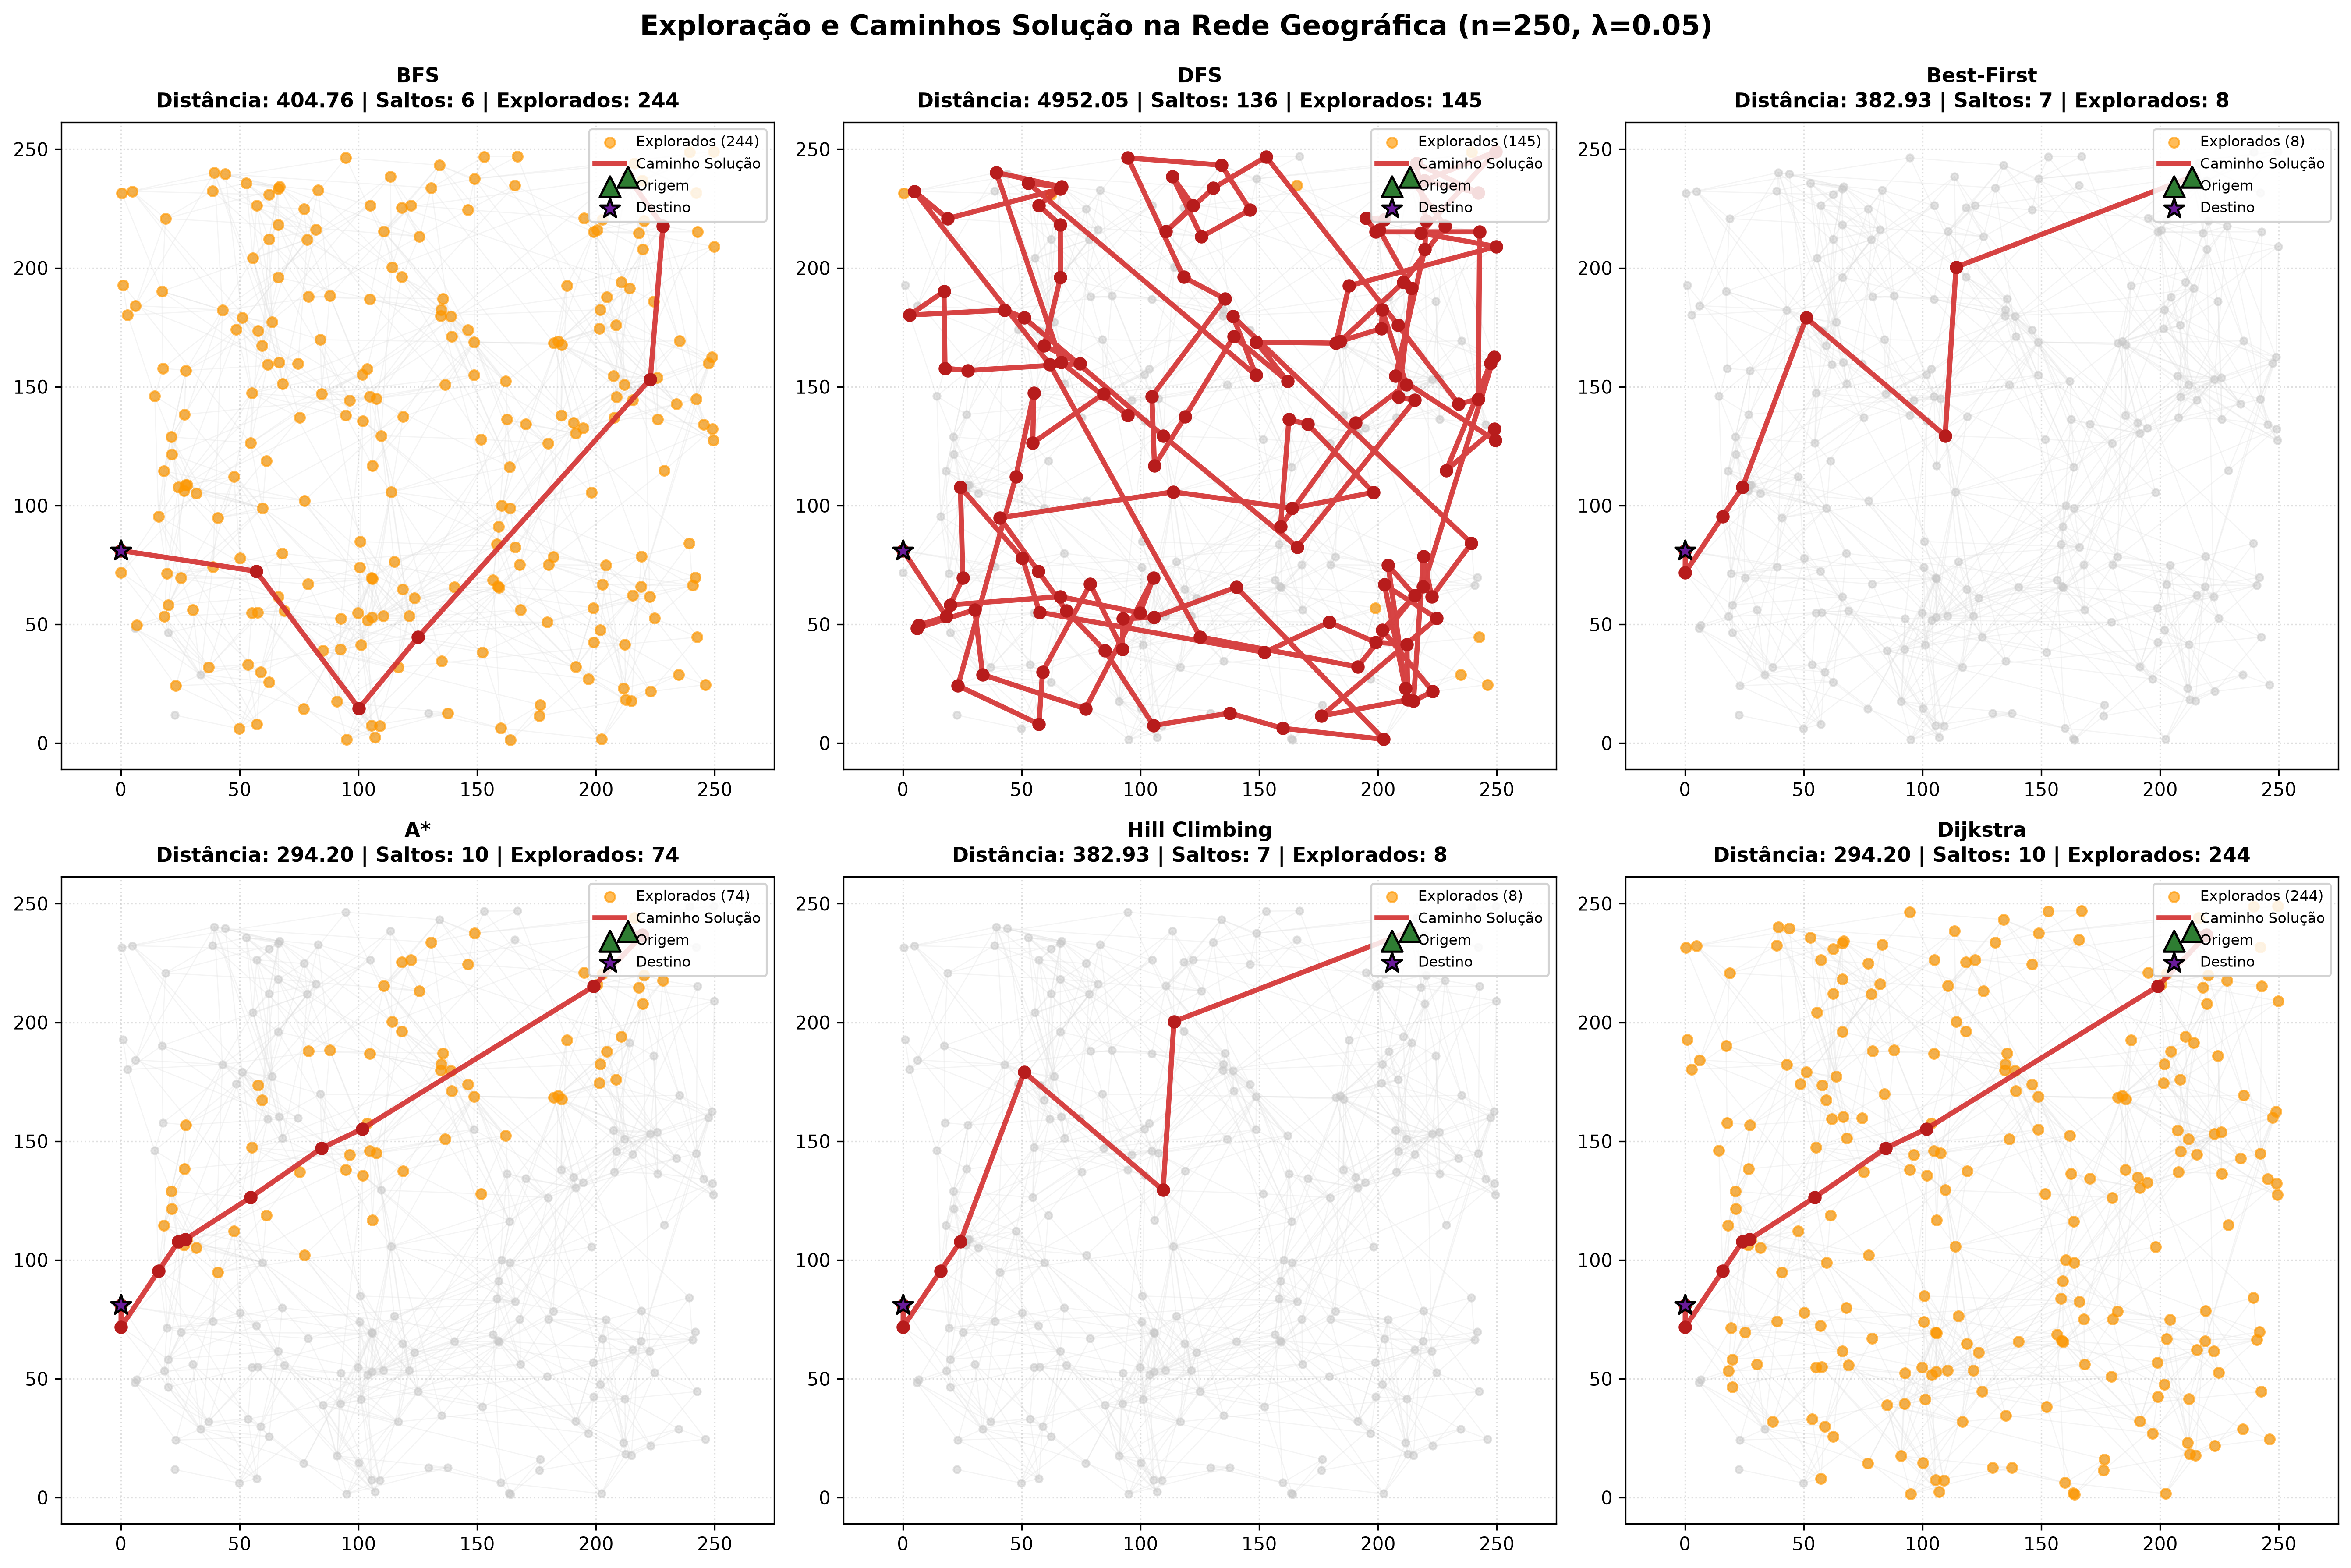
\includegraphics[width=0.98\textwidth]{figuras/visualizacao_buscas_250.png}
\caption{Painel comparativo da exploração do espaço de busca na rede geográfica ($n=250$, $\lambda=0{,}05$). Em laranja destacam-se os vértices explorados; em vermelho, o caminho final percorrido; os triângulos verdes indicam a origem e as estrelas roxas indicam o destino.}
\label{fig:visualizacao_busca}
\end{figure*}

A inspeção visual da Figura \ref{fig:visualizacao_busca} revela distinções comportamentais nítidas:
\begin{itemize}
    \item A **BFS** e o **Dijkstra** exibem expansão perfeitamente radial e isotrópica, varrendo 244 de 250 nós até interceptar o destino.
    \item O **DFS** serpenteia errante por ramos periféricos, acumulando 136 saltos e um trajeto quase 17 vezes mais longo que o ótimo.
    \item O **Best-First** e o **Hill Climbing** convergem em linha quase reta explorando apenas 8 nós, ao custo de uma rota $\approx 30\%$ subótima.
    \item O **A\*** constringe o espaço de busca dentro de uma elipse heurística direcionada, expandindo 74 nós (redução de 70\% frente ao Dijkstra) e atingindo a distância ótima idêntica de 294{,}20.
\end{itemize}

\subsection{Experimento II: Benchmark em Redes de Grande Porte (Item 4.4.ii)}

Conforme preconizado na Seção 4.4.ii do enunciado, avaliaram-se redes com $n = 2500$ vértices sob três variações de decaimento espacial:
\begin{itemize}
    \item **Rede Densa ($\lambda = 0{,}01$):** 28.370 arestas; grau médio 22{,}70; 100\% dos vértices na maior componente.
    \item **Rede Intermediária ($\lambda = 0{,}02$):** 7.439 arestas; grau médio 5{,}95; 99{,}5\% dos vértices na maior componente.
    \item **Rede Esparsa ($\lambda = 0{,}03$):** 3.398 arestas; grau médio 2{,}72; 86{,}4\% dos vértices na maior componente.
\end{itemize}

Para assegurar rigor metodológico absoluto e comparabilidade direta, selecionaram-se 10 pares distintos de vértices amostrados a partir da \textbf{interseção das maiores componentes conexas} das três redes (conjunto de 2.159 vértices mutuamente alcançáveis). Cada algoritmo foi executado com 3 repetições cronometradas com \texttt{time.perf\_counter()}.

A Tabela \ref{tab:benchmark_estatisticas} compila as métricas consolidadas (distância média, desvio padrão, saltos, nós explorados, tempo de CPU e taxa de sucesso).

\begin{table*}[!t]
\centering
\caption{Resultados consolidados do benchmark para $n = 2500$ vértices em 10 pares de teste compartilhados.}
\label{tab:benchmark_estatisticas}
\small
\begin{tabular}{llcccccc}
\toprule
\textbf{Rede} & \textbf{Algoritmo} & \textbf{Sucesso (\%)} & \textbf{Distância Média} & \textbf{Desvio Dist.} & \textbf{Saltos Médios} & \textbf{Nós Explorados} & \textbf{Tempo Médio (ms)} \\
\midrule
\multirow{6}{*}{\textbf{$\lambda = 0{,}01$}} 
 & BFS           & 100\% & 1175{,}79 & 621{,}85 & \textbf{3{,}7}  & 1022{,}4 & 3{,}01 $\pm$ 1{,}96 \\
 & DFS           & 100\% & 308938{,}49 & 135551{,}47 & 1590{,}5 & 1611{,}1 & 4{,}87 $\pm$ 3{,}26 \\
 & Best-First    & 100\% & 1227{,}75 & 648{,}58 & 4{,}5  & \textbf{5{,}5}   & \textbf{0{,}17} $\pm$ 0{,}07 \\
 & A*            & 100\% & \textbf{1028{,}58} & 542{,}34 & 6{,}3  & 27{,}4  & 0{,}66 $\pm$ 0{,}42 \\
 & Hill Climbing & 100\% & 1227{,}75 & 648{,}58 & 4{,}5  & \textbf{5{,}5}   & 0{,}07 $\pm$ 0{,}03 \\
 & Dijkstra      & 100\% & \textbf{1028{,}58} & 542{,}34 & 6{,}3  & 1026{,}9 & 9{,}81 $\pm$ 7{,}72 \\
\midrule
\multirow{6}{*}{\textbf{$\lambda = 0{,}02$}} 
 & BFS           & 100\% & 1416{,}36 & 739{,}17 & \textbf{8{,}6}  & 1034{,}9 & 1{,}30 $\pm$ 1{,}01 \\
 & DFS           & 100\% & 129370{,}72 & 29200{,}60 & 1279{,}1 & 1612{,}3 & 2{,}79 $\pm$ 1{,}19 \\
 & Best-First    & 100\% & 1353{,}33 & 716{,}10 & 11{,}7 & \textbf{13{,}9}  & \textbf{0{,}12} $\pm$ 0{,}05 \\
 & A*            & 100\% & \textbf{1116{,}98} & 596{,}61 & 11{,}8 & 102{,}3 & 0{,}70 $\pm$ 0{,}78 \\
 & Hill Climbing & \textbf{50\%}  & 1184{,}41 & 902{,}59 & 10{,}4 & 10{,}7  & 0{,}06 $\pm$ 0{,}04 \\
 & Dijkstra      & 100\% & \textbf{1116{,}98} & 596{,}61 & 11{,}8 & 1017{,}7 & 3{,}70 $\pm$ 2{,}81 \\
\midrule
\multirow{6}{*}{\textbf{$\lambda = 0{,}03$}} 
 & BFS           & 100\% & 1687{,}67 & 793{,}26 & \textbf{19{,}3} & 844{,}7  & 1{,}05 $\pm$ 0{,}93 \\
 & DFS           & 100\% & 17373{,}82  & 8197{,}96  & 244{,}6 & 1221{,}3 & 2{,}52 $\pm$ 1{,}60 \\
 & Best-First    & 100\% & 2052{,}19 & 1261{,}31 & 26{,}3 & \textbf{49{,}1}  & \textbf{0{,}24} $\pm$ 0{,}18 \\
 & A*            & 100\% & \textbf{1581{,}41} & 779{,}93 & 21{,}4 & 295{,}7 & 1{,}23 $\pm$ 1{,}23 \\
 & Hill Climbing & \textbf{0\%}   & ---      & ---      & ---    & 5{,}2   & 0{,}02 $\pm$ 0{,}01 \\
 & Dijkstra      & 100\% & \textbf{1581{,}41} & 779{,}93 & 21{,}4 & 897{,}0  & 2{,}57 $\pm$ 2{,}15 \\
\bottomrule
\end{tabular}
\end{table*}

\begin{figure}[!ht]
\centering
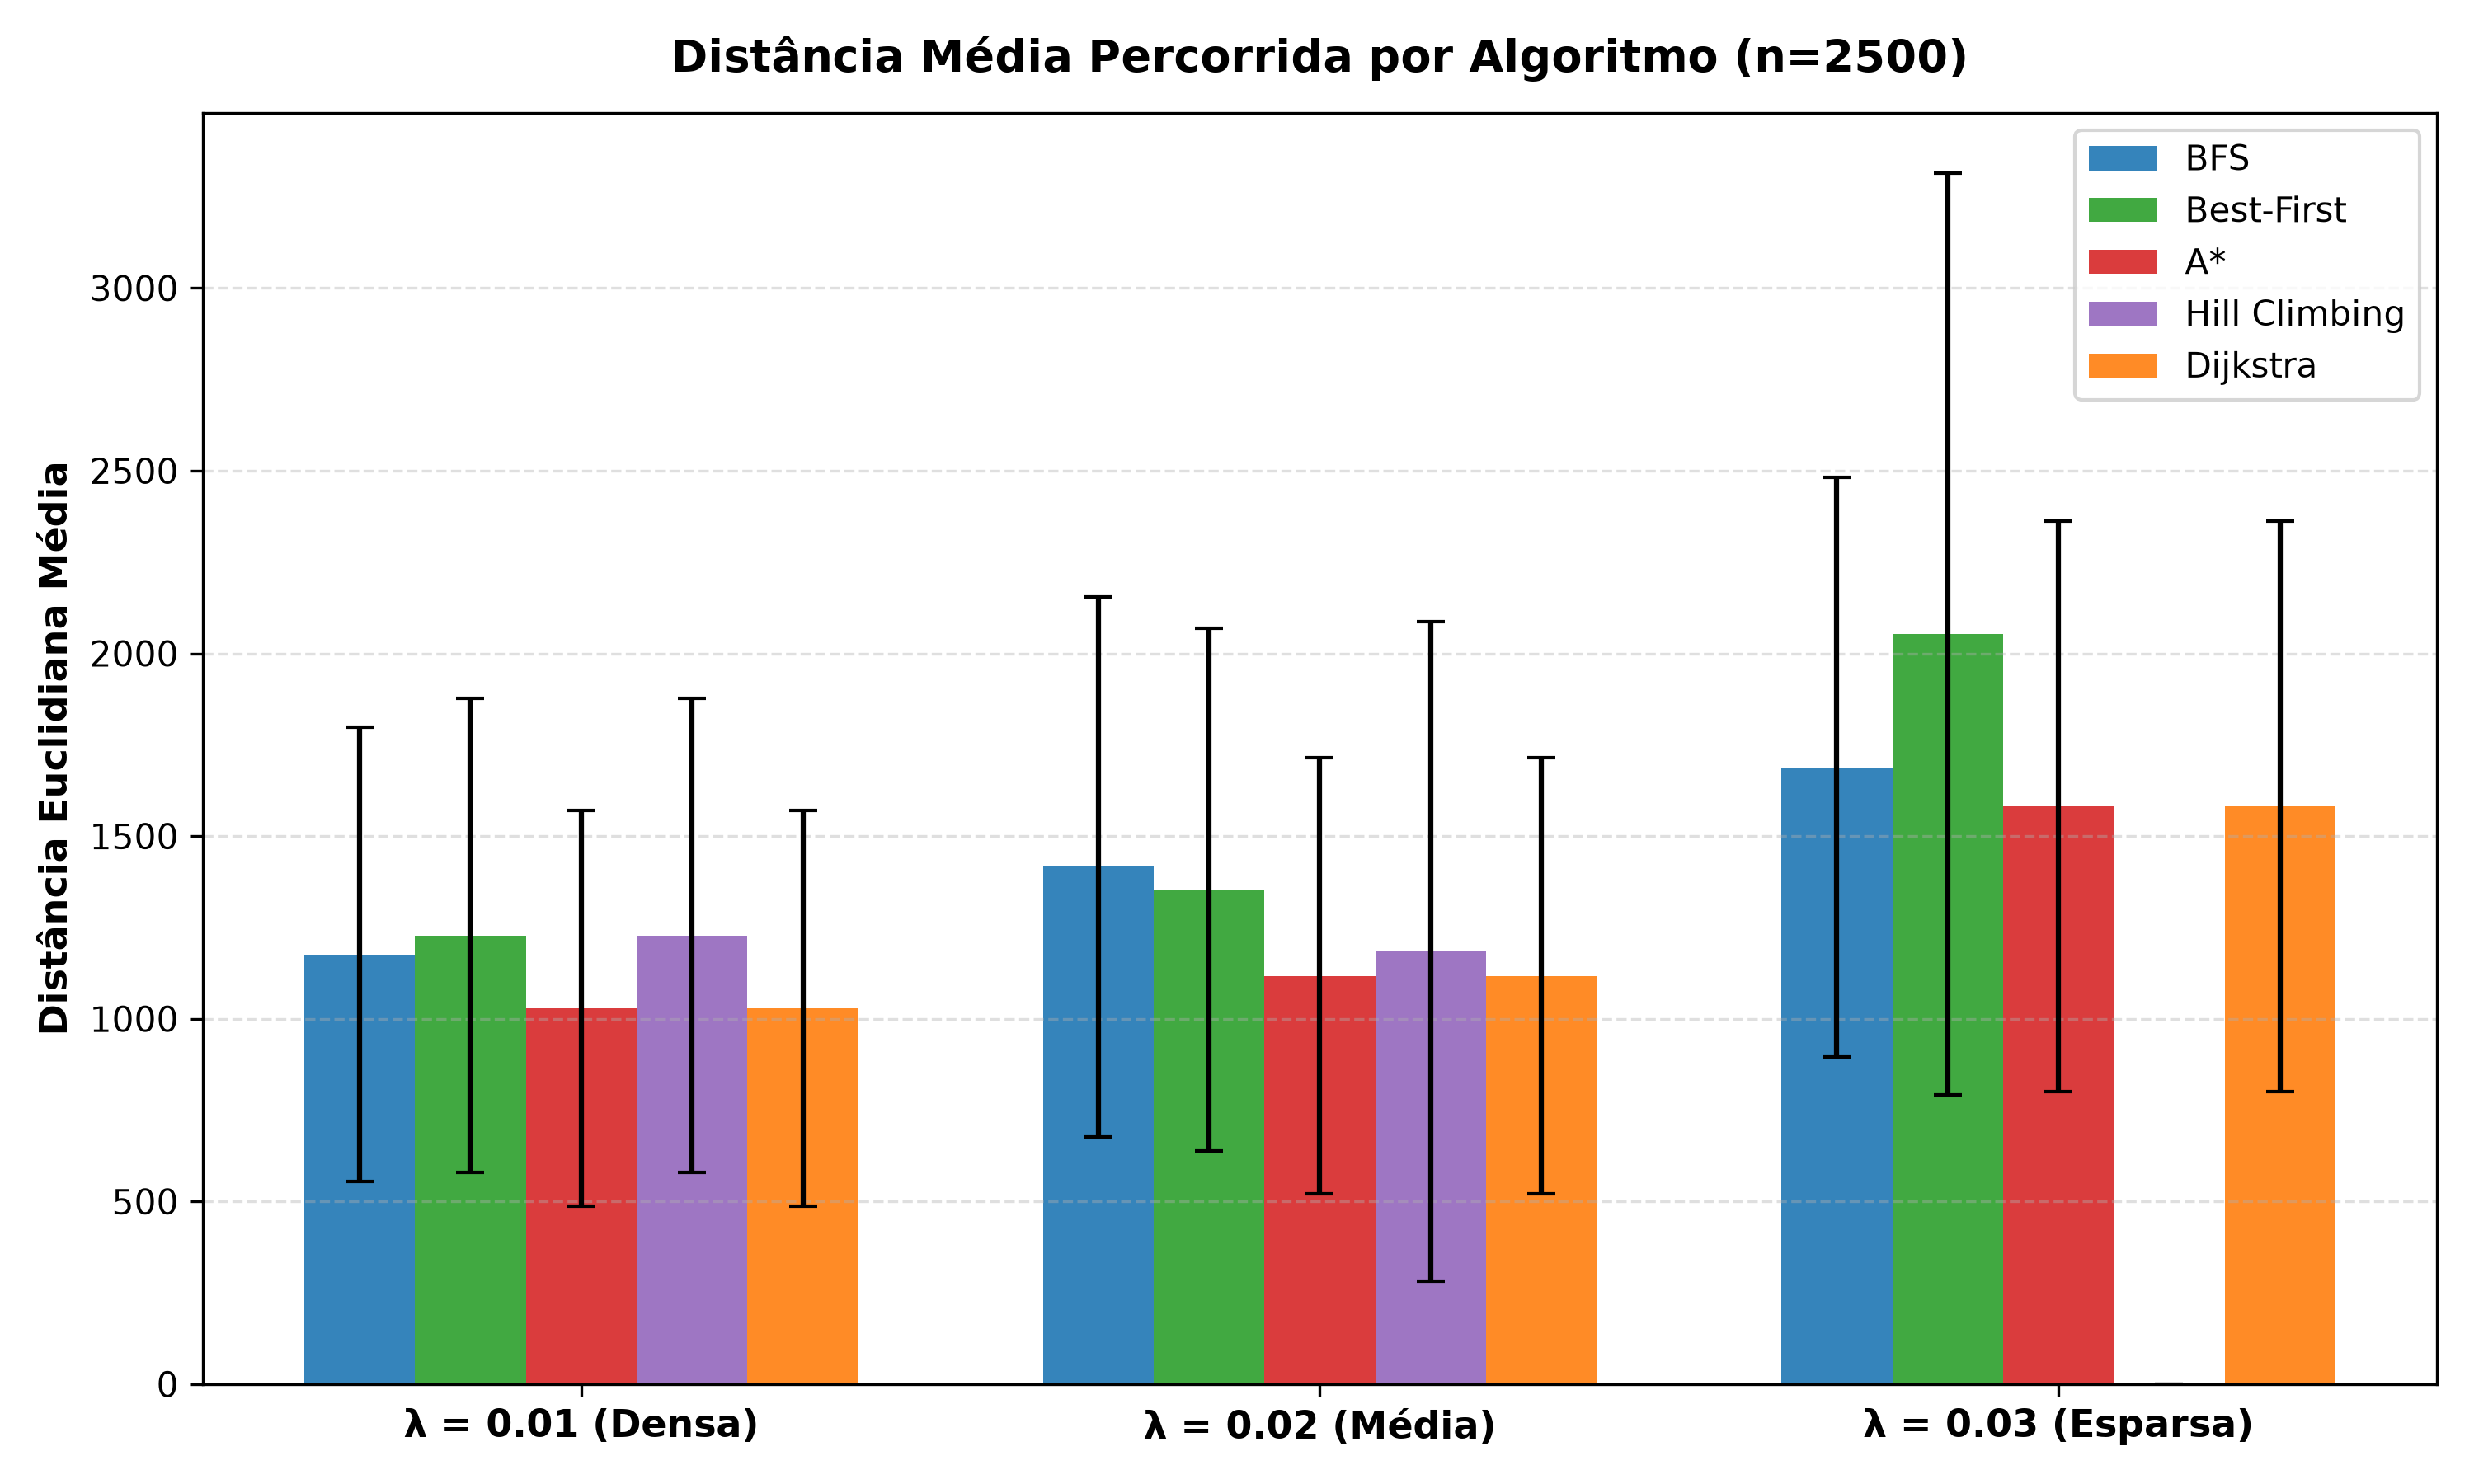
\includegraphics[width=0.48\textwidth]{figuras/benchmark_distancia.png}
\caption{Distância média percorrida pelos algoritmos sob os três regimes de $\lambda$ (DFS omitido pela discrepância de escala).}
\label{fig:distancia}
\end{figure}

\begin{figure}[!ht]
\centering
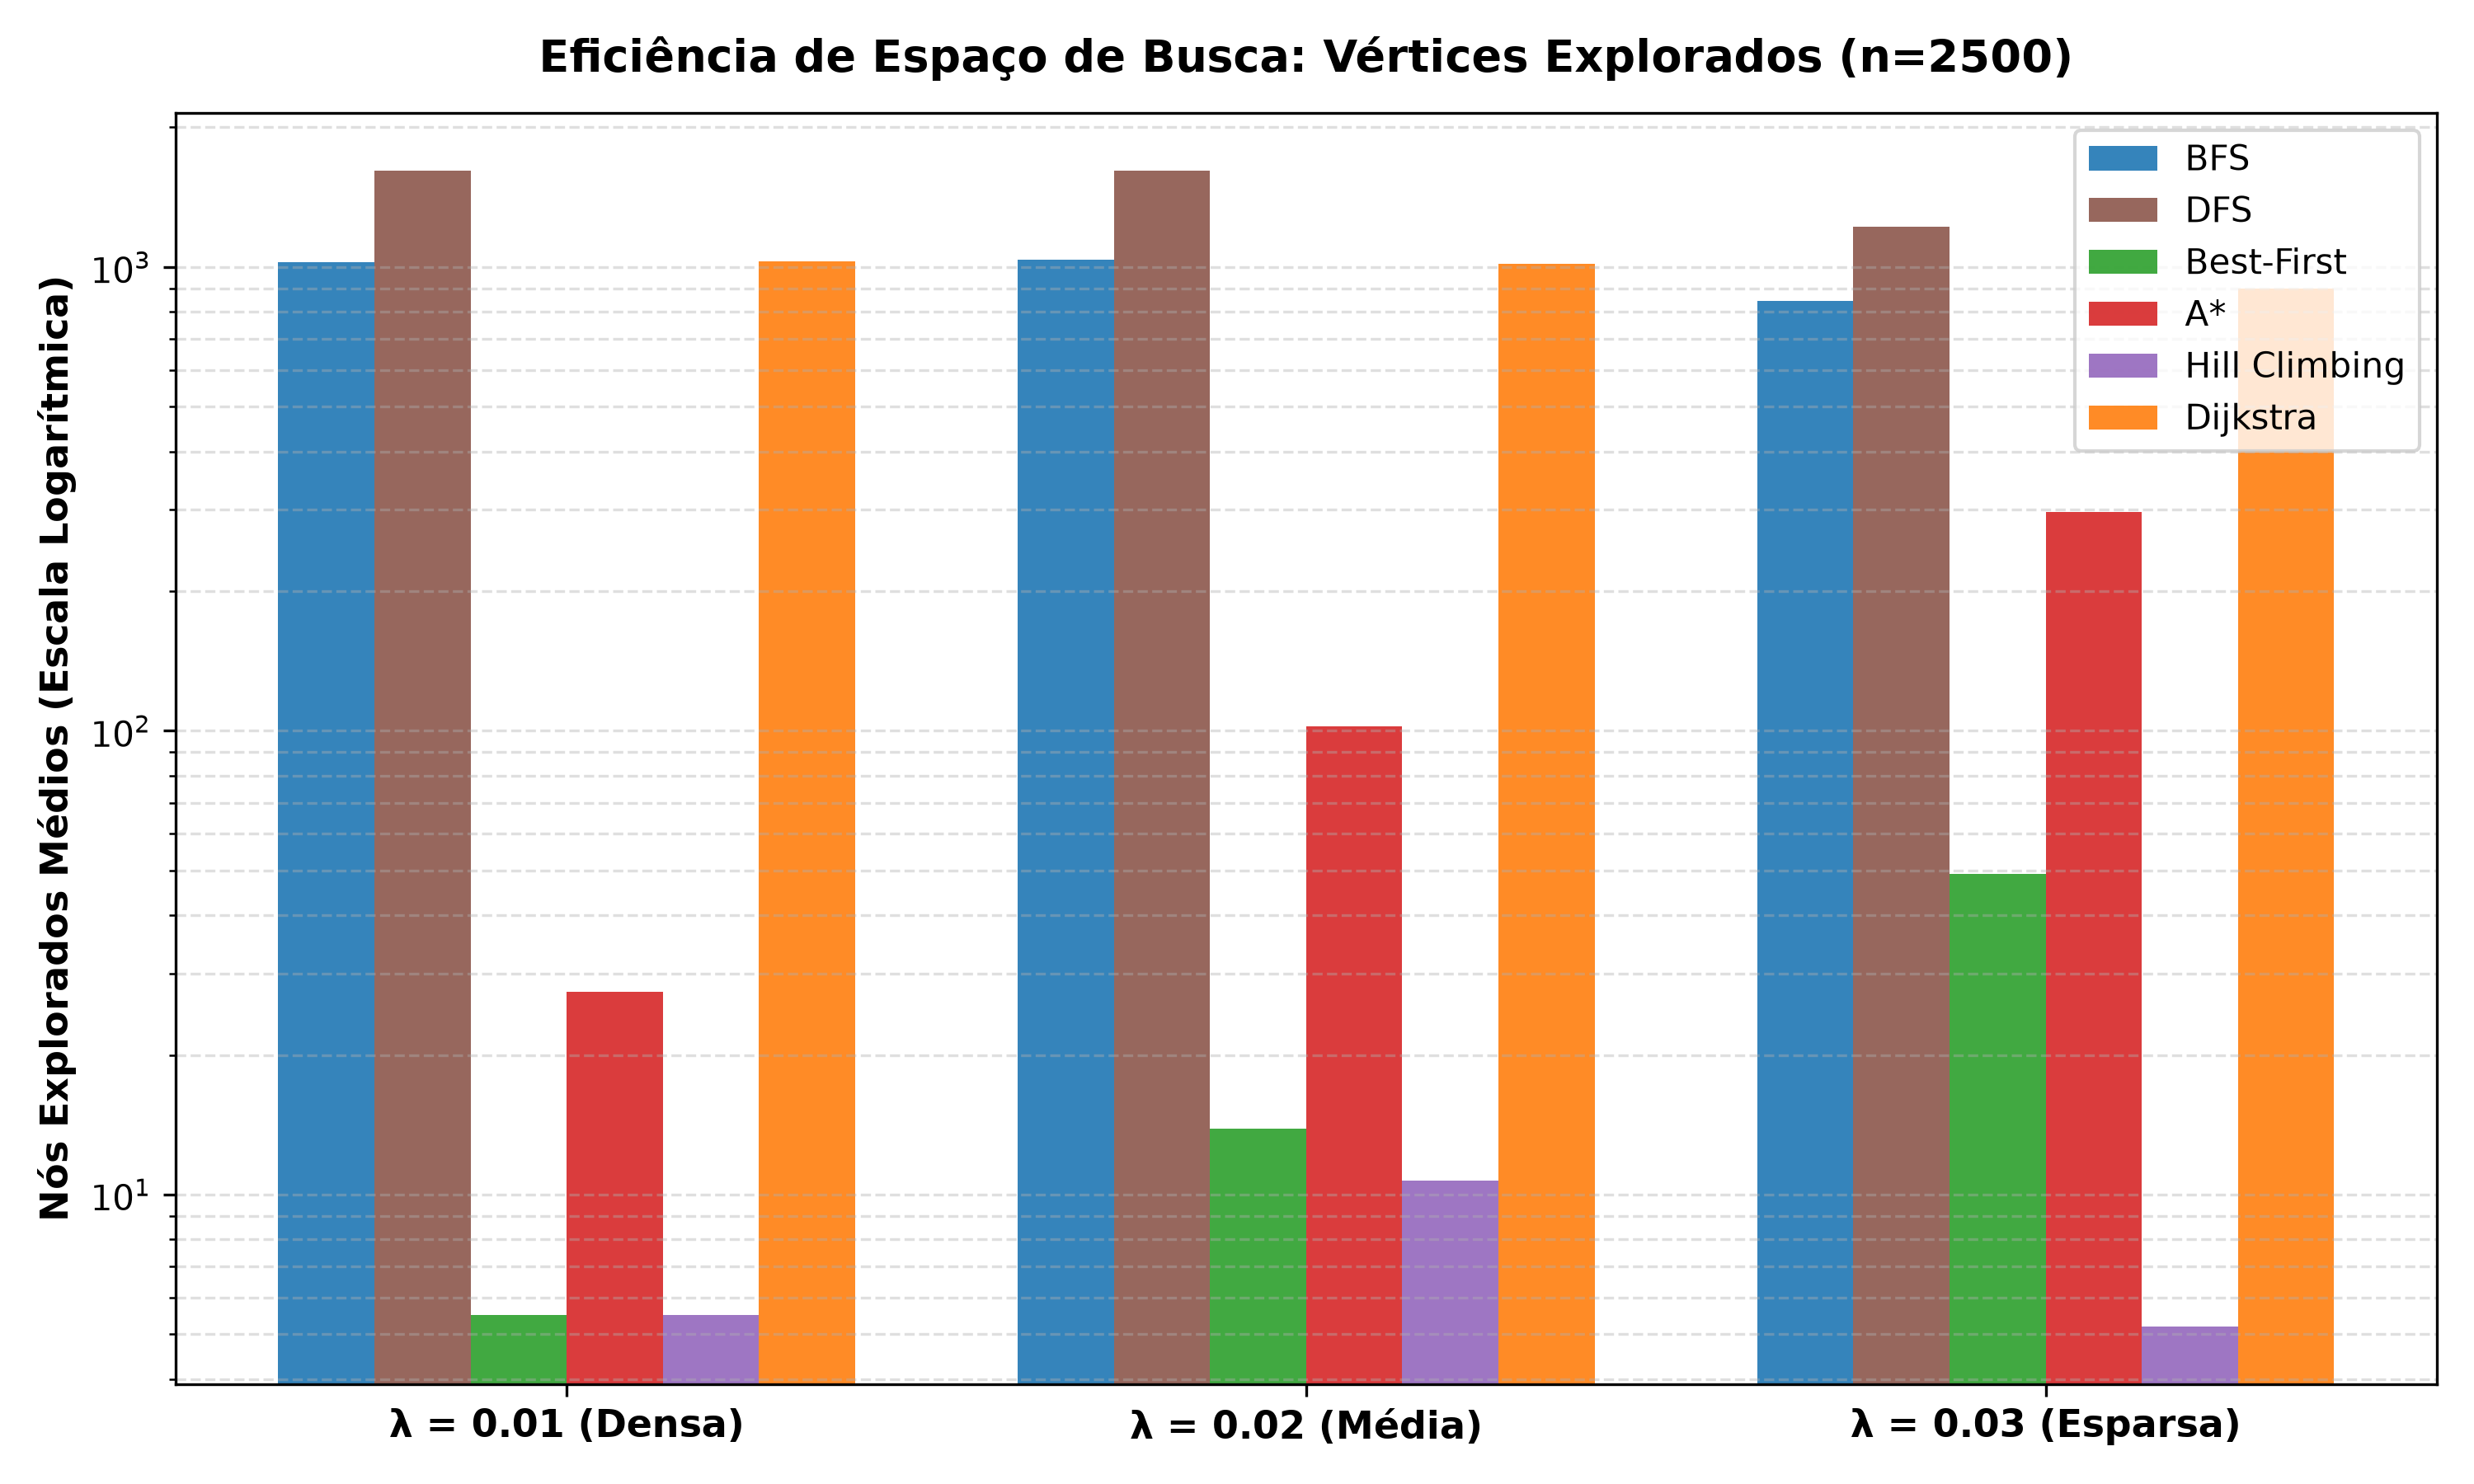
\includegraphics[width=0.48\textwidth]{figuras/benchmark_explorados.png}
\caption{Vértices explorados médios em escala logarítmica, evidenciando a expressiva economia de estados do A* e Best-First.}
\label{fig:explorados}
\end{figure}

\subsection{Experimento III: Comparação Sistemática entre A* e Dijkstra (Item 4.4.iii)}

A comparação direta entre o A* e o Dijkstra (Figura \ref{fig:astar_dijkstra}) evidencia o impacto da função heurística sobre o mesmo objetivo de minimização ótima de custo:
\begin{itemize}
    \item \textbf{Caminho e Custo:} Em todas as 30 instâncias testadas (3 redes $\times$ 10 pares), o A* e o Dijkstra obtiveram \textbf{rigorosamente os mesmos caminhos ótimos e as mesmas distâncias finais acumuladas}.
    \item \textbf{Poda de Espaço de Busca:} Na rede densa ($\lambda = 0{,}01$), o Dijkstra expandiu 1026{,}9 nós contra apenas 27{,}4 nós do A* --- uma redução de \textbf{37{,}5 vezes} (economia de 97{,}3\% dos vértices). Na rede intermediária ($\lambda = 0{,}02$), a razão foi de 10{,}0 vezes (1017{,}7 vs. 102{,}3). Na rede esparsa ($\lambda = 0{,}03$), onde os caminhos são canalizados por rotas únicas, a redução foi de 3{,}0 vezes (897{,}0 vs. 295{,}7).
    \item \textbf{Tempo de Execução:} Na rede densa com elevado número de arestas incidentes, a poda do A* refletiu-se em tempo médio de 0{,}66 ms contra 9{,}81 ms do Dijkstra (aceleração de 14{,}8 vezes).
\end{itemize}

\begin{figure}[!ht]
\centering
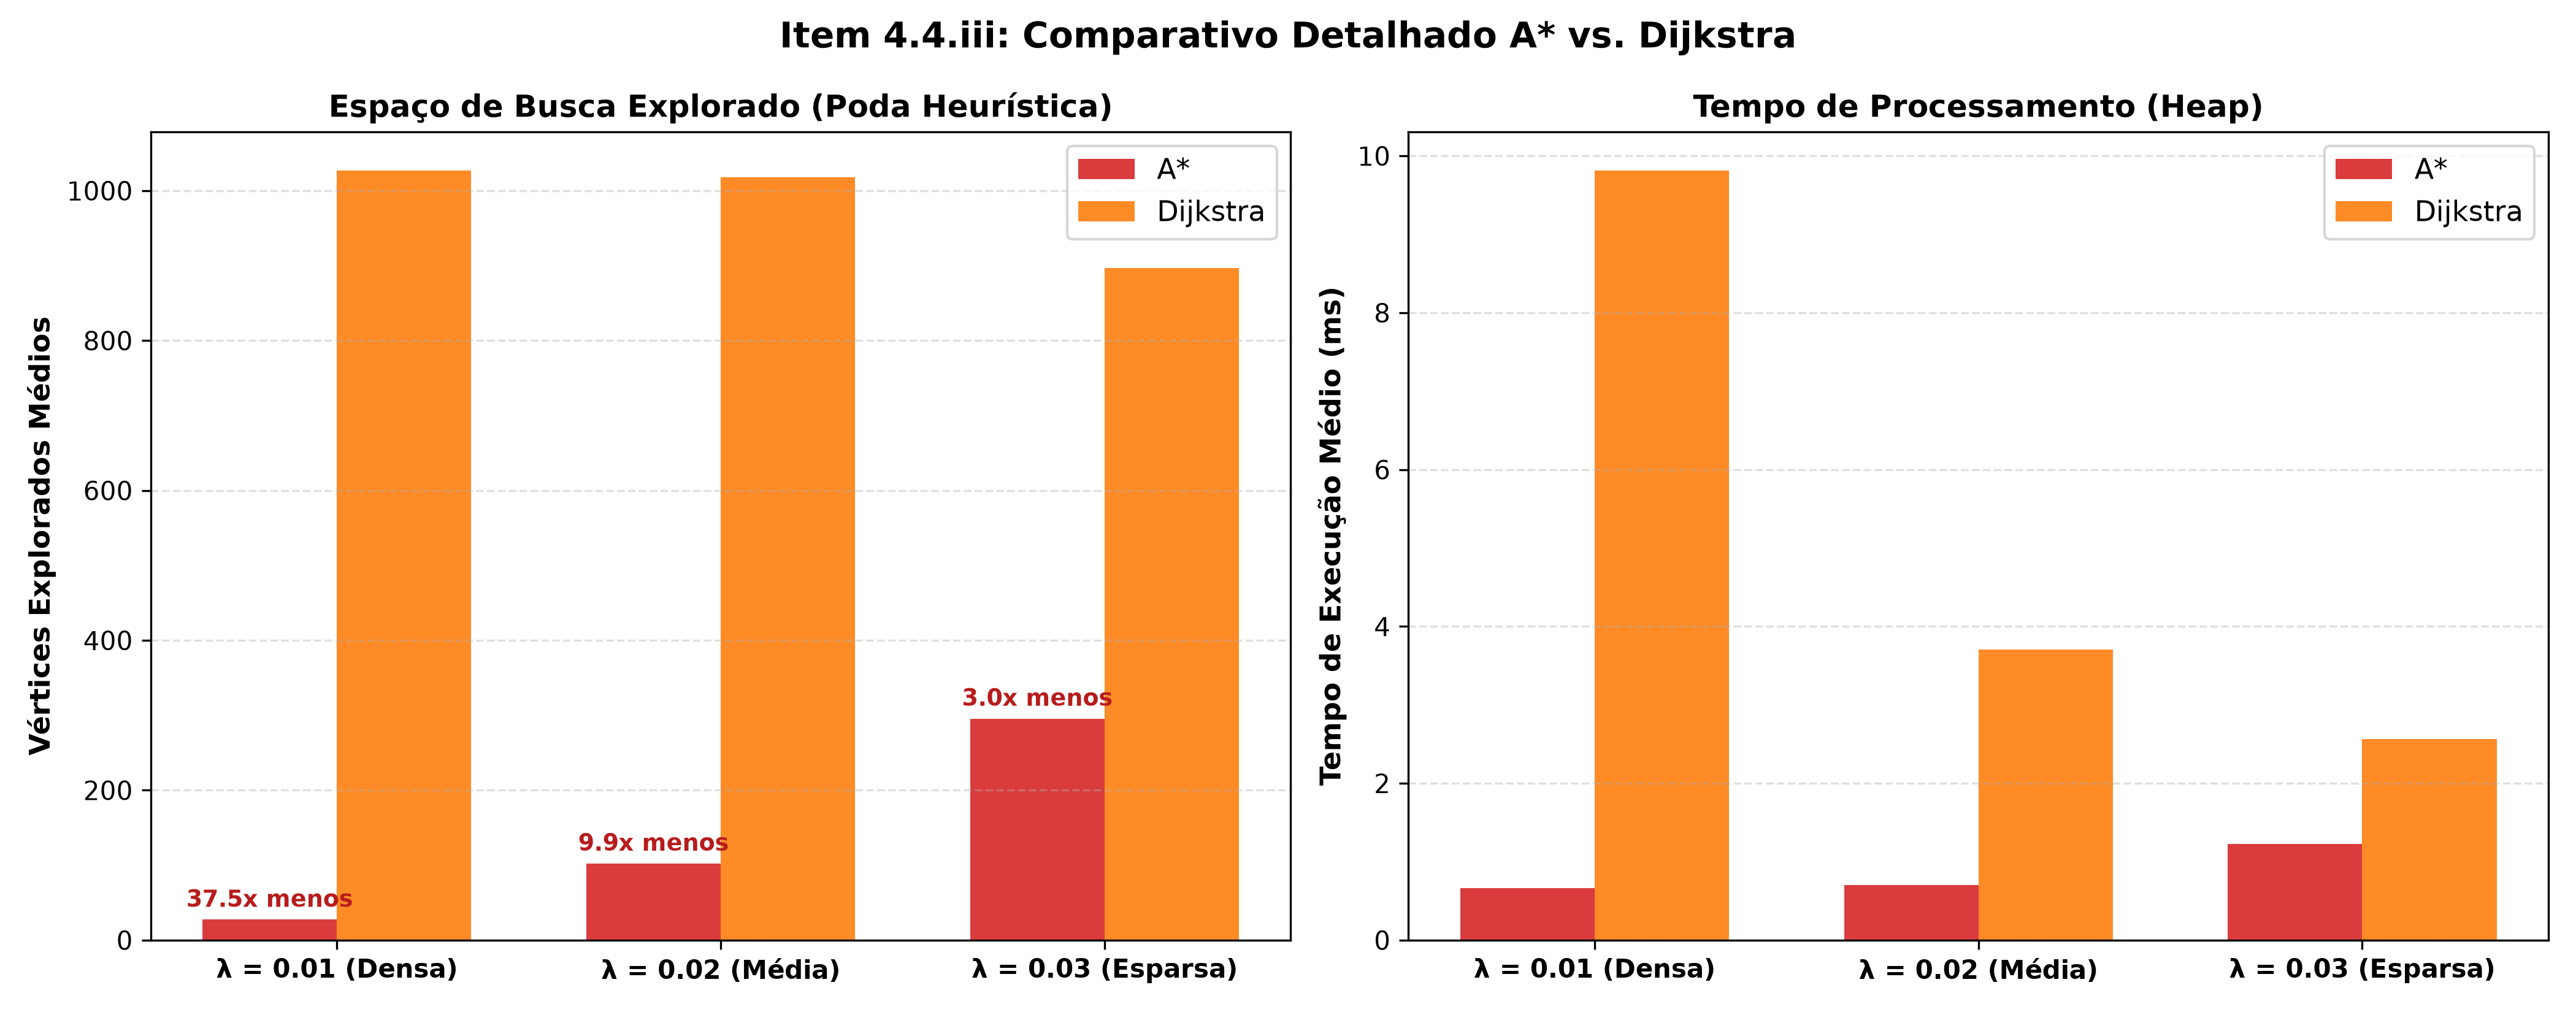
\includegraphics[width=0.49\textwidth]{figuras/comparativo_astar_dijkstra.png}
\caption{Comparação formal entre A* e Dijkstra (Item 4.4.iii): vértices explorados e tempo de processamento.}
\label{fig:astar_dijkstra}
\end{figure}

\section{Discussão dos Resultados e das Visualizações}
\label{sec:discussao}

\subsection{O Fenômeno do Colapso do Hill Climbing}

Um dos resultados teóricos mais expressivos obtidos no trabalho é ilustrado na Figura \ref{fig:sucesso}, que documenta a transição de fase da taxa de sucesso do Hill Climbing sem backtracking:
\begin{itemize}
    \item Em $\lambda = 0{,}01$, com grau médio de 22{,}70, a alta conectividade espacial garante múltiplos caminhos circundantes; assim, a descida de gradiente euclidiano local não encontrou barreiras, atingindo 100\% de sucesso.
    \item Em $\lambda = 0{,}02$, a emergência de lacunas topológicas fez com que 50\% das buscas colidissem com vértices cujo conjunto de vizinhos não oferecia avanço em direção ao alvo ($h(v) \ge h(\text{atual})$), encerrando a busca prematuramente.
    \item Em $\lambda = 0{,}03$, sob grau médio de 2{,}72, a topologia exibe gargalos estruturais e sinuosidades severas. O algoritmo falhou em \textbf{100\% dos pares analisados} (0\% de sucesso), confirmando que a ausência de retrocesso inviabiliza a busca local em redes esparsas não-convexas.
\end{itemize}

\begin{figure}[!ht]
\centering
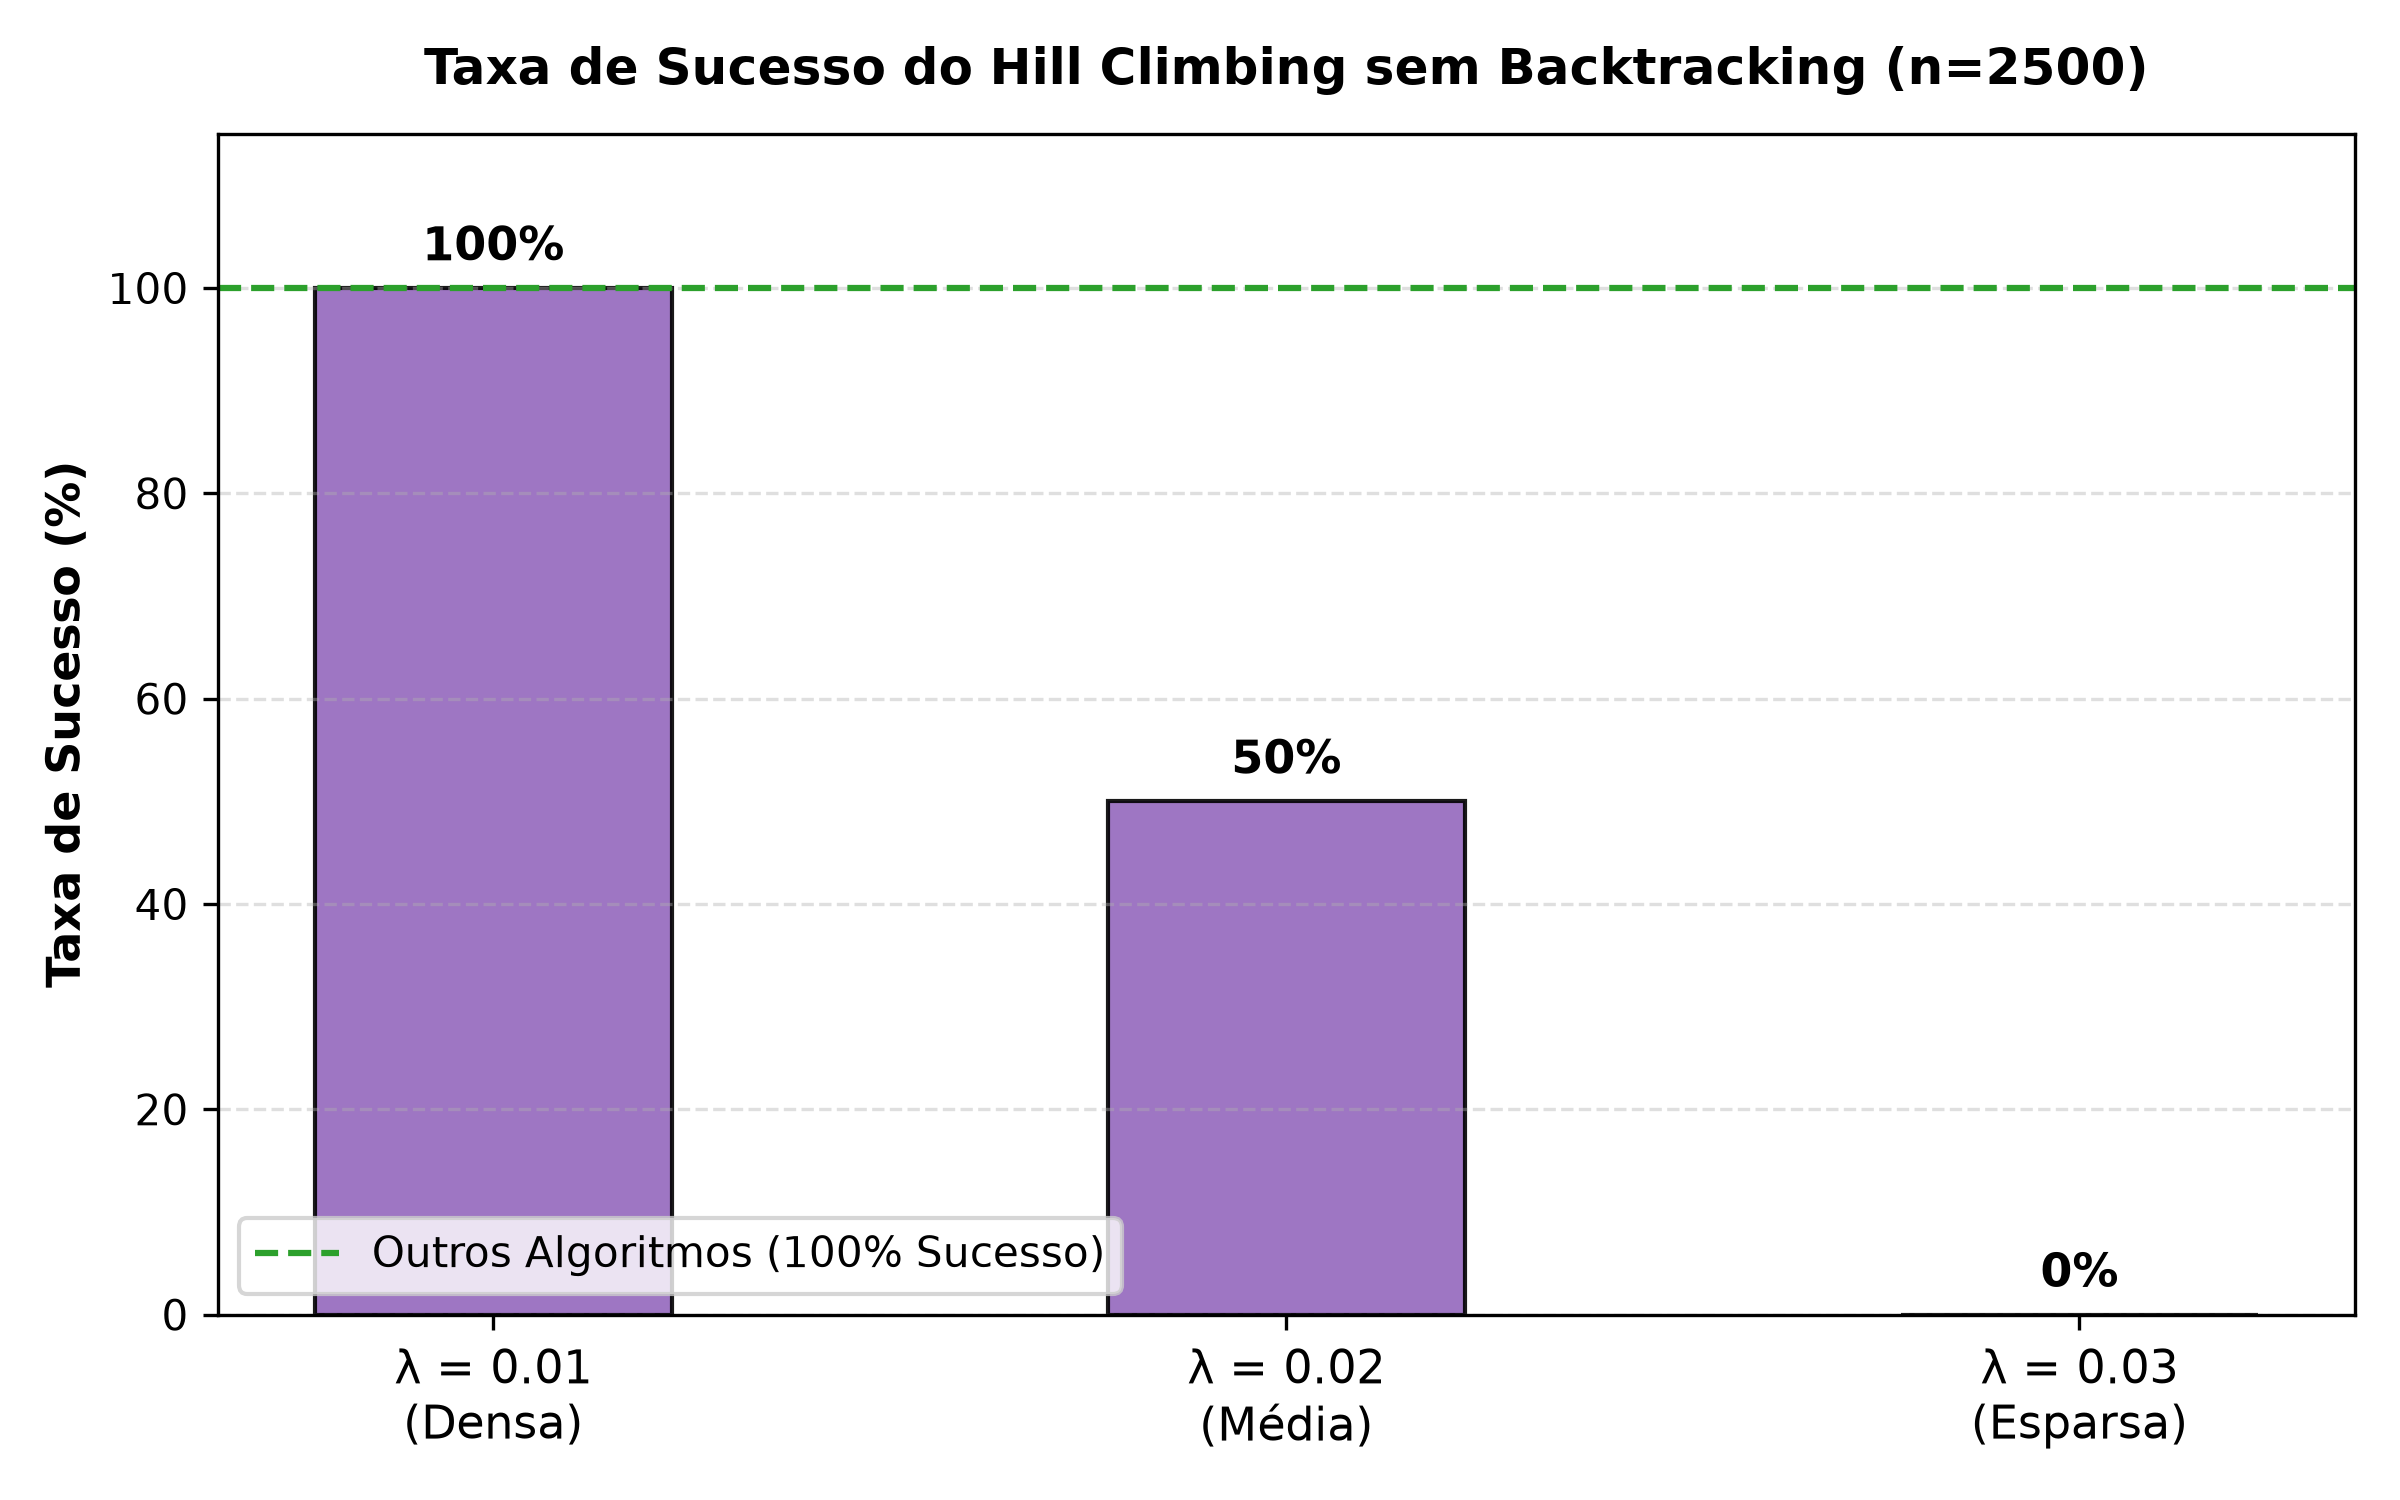
\includegraphics[width=0.45\textwidth]{figuras/benchmark_sucesso.png}
\caption{Taxa de sucesso do Hill Climbing em função de $\lambda$, ilustrando a quebra de completude induzida pela esparsidade.}
\label{fig:sucesso}
\end{figure}

\subsection{Inviabilidade da Busca em Profundidade em Grafos Ponderados}

A DFS exibiu comportamento patológico em todas as configurações. Na rede $\lambda = 0{,}01$, enquanto o trajeto ótimo possuía custo 1028{,}58 e 6{,}3 saltos, o DFS percorreu em média 1590{,}5 saltos acumulando distância média de 308.938{,}49 (fator de degradação de $\approx 300\times$). Esse fenômeno decorre da natureza do DFS: ao aprofundar-se por arestas arbitrárias, o algoritmo acumula nós distantes em ziguezague antes de esgotar ramos, sendo plenamente desaconselhado para aplicações de roteamento.

\subsection{Trade-off entre Best-First e A*}

O Best-First demonstrou extraordinária celeridade: explorou em média apenas 5{,}5 nós em $\lambda = 0{,}01$ e 49{,}1 nós em $\lambda = 0{,}03$, operando na faixa de 0{,}1 a 0{,}2 milissegundos. No entanto, sua miopia em relação ao custo percorrido $g(n)$ acarretou distâncias 19\% a 30\% superiores ao ótimo. Em contrapartida, o A* consumiu frações adicionais de milissegundo para garantir a rota ótima global. Para sistemas de missão crítica em tempo real com hardware ultralimitado, o Best-First desponta como heurística viável; contudo, para logística e transporte, o A* compensa amplamente seu modesto custo adicional.

\section{Conclusões}
\label{sec:conclusao}

Este projeto implementou e avaliou rigorosamente algoritmos de busca clássicos e heurísticos em Redes Geográficas estocásticas. As principais conclusões são:
\begin{enumerate}
    \item O modelo estocástico baseado em decaimento exponencial $P(u \to v) = e^{-\lambda s_{uv}}$ reproduziu satisfatoriamente as características topológicas de redes espaciais reais.
    \item A heurística euclidiana $h(n)$ atendeu integralmente aos critérios de admissibilidade e consistência, conferindo ao A* redução de até 97\% no espaço explorado em relação ao Dijkstra, sem qualquer perda de otimalidade.
    \item Algoritmos de otimização local pura (Hill Climbing sem backtracking) são altamente vulneráveis à esparsidade da rede, colapsando para 0\% de sucesso em grafos com grau médio reduzido.
    \item O algoritmo A* consolidou-se como a abordagem superior para problemas de navegação espacial, equilibrando otimalidade exata de custo e parcimônia computacional.
\end{enumerate}

\begin{thebibliography}{99}

\bibitem{russell2020}
S.~Russell and P.~Norvig,
\emph{Artificial Intelligence: A Modern Approach}, 4th~ed.
Hoboken, NJ: Pearson, 2020.

\bibitem{dijkstra1959}
E.~W. Dijkstra,
``A note on two problems in connexion with graphs,''
\emph{Numerische Mathematik}, vol.~1, no.~1, pp. 269--271, 1959.

\bibitem{hart1968}
P.~E. Hart, N.~J. Nilsson, and B.~Raphael,
``A formal basis for the heuristic determination of minimum cost paths,''
\emph{IEEE Transactions on Systems Science and Cybernetics}, vol.~4, no.~2, pp. 100--107, 1968.

\bibitem{barthelemy2011}
M.~Barthélemy,
``Spatial networks,''
\emph{Physics Reports}, vol.~499, no. 1-3, pp. 1--101, 2011.

\bibitem{newman2010}
M.~Newman,
\emph{Networks: An Introduction}.
Oxford: Oxford University Press, 2010.

\end{thebibliography}

\end{document}
